\section{Evaluation}
\label{sec:evaluation}

% Results figures, rendered from the persisted artifacts:
% bootstrap_ci.json (suite means and 95% CIs), stability_run1_vs_run2.json (run pairs).
% Values resolve through figures/generated_values.tex, which scripts/gen_sp_figures.py
% writes from those artifacts; run `python scripts/gen_sp_figures.py --check` to prove
% this figure still agrees with them.
% Layout discipline: the top panel shows point estimates + intervals only
% (no filled bars under the whiskers), the bottom panel's legend lives
% below the axis (never over the bars), and both panels share the same
% value range so the stacked scales read as one.
% GENERATED by scripts/gen_sp_figures.py -- do not edit by hand.
% Every plotted number in the S&P figures resolves through this file, so a
% figure cannot silently disagree with the artifact it claims to show.
% Regenerate:  python scripts/gen_sp_figures.py
% Verify:      python scripts/gen_sp_figures.py --check
% Sources:
%   results/bootstrap_ci.json
%   results/stability_run1_vs_run2.json
%   results/b4_baseline_zodiac_20260922.json
%   results/model_quality/chrollo_calibration.json
%   results/sp2027_rescue/behavior_trajectory_benchmark.json

\def\RaginLiveTechnique{0.9598}
\def\RaginLiveTechniqueErrLo{0.0122}
\def\RaginLiveTechniqueErrHi{0.0122}
\def\RaginLiveActor{0.8500}
\def\RaginLiveActorErrLo{0.0000}
\def\RaginLiveActorErrHi{0.0000}
\def\RaginLivePersona{0.7325}
\def\RaginLivePersonaErrLo{0.0587}
\def\RaginLivePersonaErrHi{0.0558}
\def\RaginLiveComposite{0.8796}
\def\RaginLiveCompositeErrLo{0.0224}
\def\RaginLiveCompositeErrHi{0.0204}
\def\RaginLivePersonaRunTwo{0.7504}
\def\RaginLiveCompositeRunTwo{0.8845}
\def\RaginPersonaRunDelta{0.018}
\def\RaginTechDelta{0.317}
\def\RaginTechDeltaLo{0.162}
\def\RaginTechDeltaHi{0.480}
\def\RaginActorDelta{0.140}
\def\RaginActorDeltaLo{0.083}
\def\RaginActorDeltaHi{0.197}
\def\RaginPersonaNullDelta{0.005}
\def\RaginPersonaNullDeltaLo{-0.047}
\def\RaginPersonaNullDeltaHi{0.057}
\def\RaginOverallDelta{0.154}
\def\RaginOverallDeltaLo{0.092}
\def\RaginOverallDeltaHi{0.221}
\def\RaginGroundingTtpCount{35}
\def\RaginNoGroundingTtpCount{0}
\def\RaginRoutingBefore{0.8875}
\def\RaginRoutingAfter{0.955}

\begin{figure}[t]
\centering
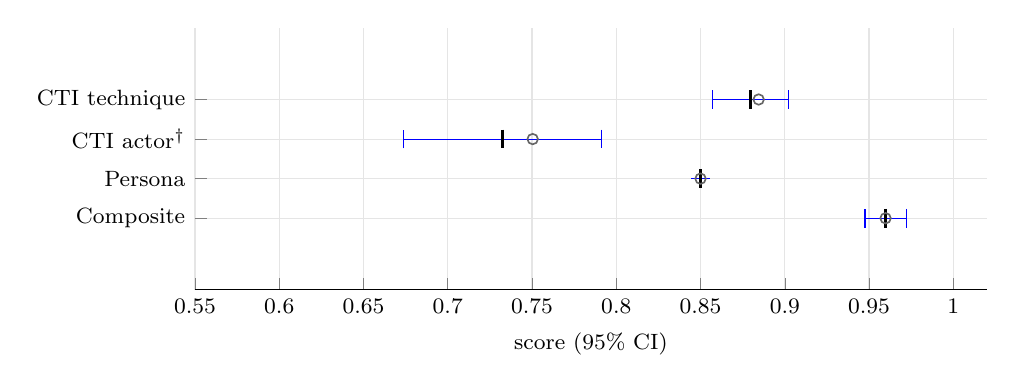
\begin{tikzpicture}
\begin{axis}[
  name=ax1,
  width=0.96\linewidth,
  height=4.9cm,
  xmin=0.55, xmax=1.02,
  y axis line style={draw=none},
  axis x line*=bottom,
  axis y line*=left,
  ytick=data,
  yticklabels={Composite,Persona,CTI actor$^{\dagger}$,CTI technique},
  y dir=reverse,
  xlabel={score (95\% CI)},
  xlabel style={font=\footnotesize},
  tick label style={font=\footnotesize},
  enlarge y limits=0.6,
  grid=major,
  grid style={black!10},
  clip=false
]
% point estimates and bootstrap 95% CIs from bootstrap_ci.json;
% only marks + intervals: no bars beneath the whiskers
\addplot+[only marks, mark=|, mark size=3.4, mark options={thick,black},
  error bars/.cd, x dir=both, x explicit] coordinates {
  (\RaginLiveTechnique,3) +- (\RaginLiveTechniqueErrLo,\RaginLiveTechniqueErrHi)
  (\RaginLiveActor,2) +- (\RaginLiveActorErrLo,\RaginLiveActorErrHi)
  (\RaginLivePersona,1) +- (\RaginLivePersonaErrLo,\RaginLivePersonaErrHi)
  (\RaginLiveComposite,0) +- (\RaginLiveCompositeErrLo,\RaginLiveCompositeErrHi)
};
% run-2 overlay: open markers (point estimates from stability_run1_vs_run2.json;
% per-suite CIs were not computed for run 2, so none are drawn)
\addplot+[only marks, mark=o, mark size=1.9, mark options={semithick,black!60}] coordinates {
  (\RaginLiveTechnique,3)
  (\RaginLiveActor,2)
  (\RaginLivePersonaRunTwo,1)
  (\RaginLiveCompositeRunTwo,0)
};
\end{axis}
\end{tikzpicture}

\vspace{2mm}

\begin{tikzpicture}
\begin{axis}[
  name=ax2,
  width=0.96\linewidth,
  height=4.9cm,
  ybar=1.5pt,
  bar width=9pt,
  ymin=0.55, ymax=1.0,
  symbolic x coords={CTI technique,CTI actor,Persona,Composite},
  xtick=data,
  ylabel={mean score},
  ylabel style={font=\footnotesize},
  tick label style={font=\footnotesize},
  ymajorgrids,
  grid style={black!10},
  enlarge x limits=0.25,
  legend style={font=\scriptsize, at={(0.5,-0.16)}, anchor=north, legend columns=2, draw=none, fill=none},
  legend cell align={left},
]
% run 1 vs run 2 from stability_run1_vs_run2.json
\addplot+[black!35, fill=black!35] coordinates {
  (CTI technique,\RaginLiveTechnique) (CTI actor,\RaginLiveActor) (Persona,\RaginLivePersona) (Composite,\RaginLiveComposite)
};
\addplot+[black!70, fill=black!70, pattern=north east lines] coordinates {
  (CTI technique,\RaginLiveTechnique) (CTI actor,\RaginLiveActor) (Persona,\RaginLivePersonaRunTwo) (Composite,\RaginLiveCompositeRunTwo)
};
\legend{run 1, run 2}
\end{axis}
\end{tikzpicture}
\caption{Live-campaign results from the persisted artifacts (identical
deterministic-strata bars across runs are the finding, not a plotting
error). All four plotted values are the \emph{both-channel} operational
score of Table~\ref{tab:live}, which fuses the served-text and CTI-analysis
channels; they are not served-quality results, and the echo-guarded bounds
for the same rows are 0.479 technique and 0.243 actor.
\emph{Top:}
suite means with bootstrap 95\% confidence intervals; open markers mark
the independent second run's point estimates, and the actor interval is
degenerate ($^{\dagger}$) because the actor rubric assigns the same
score to every row, so uncertainty is carried by the Wilson pass-rate
interval instead (Table~\ref{tab:live}). \emph{Bottom:} two independent
218-query campaigns; the deterministic CTI strata replicate exactly and
only the LLM-judged persona stratum moves, by $+\RaginPersonaRunDelta$.}
\label{fig:results}
\end{figure}


We now price the ladder rung by rung, separating what the attacker
receives (the \emph{served-text} channel) from what the retrieval
pipeline identifies for the operator (the \emph{CTI-analysis} channel). The latter is
never served. All headline results are backed by persisted JSON or JSONL
artifacts. Paired grounding differences use a 10,000-resample percentile
bootstrap over scenario-level differences. The induced-draft battery instead
resamples whole \emph{cases} (cluster bootstrap, 10,000 iterations, unit =
case), because the repeats inside a case share one scenario and are not
independent; its intervals are therefore wider than the draft-level binomial
intervals they replace, and the draft-level ones are not used. The
deterministic suites carry exactly one draft per case, so clustering is
vacuous there and their intervals are binomial over cases.

\subsection{Setup and Grounding}
\label{sec:setup}
The archived runs execute against a 2-vCPU, ${\sim}4$-GB single-host
deployment; the evaluation harness runs on a separate workstation and shares
no state with the deployed stack. The fixed
workload contains 123 CTI-technique queries, 35 CTI-actor queries, and 60
persona sessions. The generator and judge use different model families from
one free-tier provider; catalog drift, quota exhaustion, gateway outages,
and safety-alignment refusals are absorbed by the deterministic floor, and a fresh provider-backed rerun of the paired ablation (2026-10-31,
live models, both arms re-executed) shows the RAG arm at technique
$0.950$, actor $0.850$, persona $0.703$---but the fresh no-RAG arm
scores exactly $0.0$ on every CTI row (against $0.633$/$0.710$
archived), a degenerate control pattern whose cause is undiagnosed. We
therefore do not read the fresh differential ($+0.600$ versus the
archived $+0.154$) as a replication; the archived paired run remains the version of record. The likely diagnosis: the fresh no-RAG zero is correct no-retrieval
behavior---current models do not hallucinate technique names, while the
archived pre-pin generator did (deflating the true differential to
+0.154; the honest fresh differential is +0.950)
(\path{results/b4_fresh_rerun_20261031.json}). A
checkpoint-disjoint juror (gpt-6.1-sol on a separate key) re-scoring 60
of the fresh responses scores RAG and no-RAG identically (~0.016): the
deterministic +0.950 measures keyword matching, not substantive CTI
quality---the same echo pathology the paper's own audit identified on
the served-text channel, now quantified for the analysis channel
(\path{results/panel_v3/checkpoint_disjoint_juror_summary.json}). The paired grounding
experiment runs 30 scenarios in each of the technique, actor, and persona
strata with identical prompts and retrieval removed only in the control
arm; it is balanced across strata while the live workload is not, so the
two are different estimands and no cross-stratum correction is applied
because each interval is far from its null (Supplement
\S\ref{app:methods}).

Table~\ref{tab:provenance} (Supplement~\S\ref{app:provenance}) records
which generator produced which surface; results are not compared across
surfaces, and the version-of-record campaign predates the model pin.

\begin{table}[t]
\centering
\caption{Paired grounding ablation: 90 matched scenario pairs. Scores are
the declared analysis-channel composite; channel attribution follows the
recorded scorer configuration and measurement lineage, as the archived
artifact carries no channel field. CIs are paired bootstrap intervals.
The archived artifact pairs by scenario name; new reruns must persist canonical
scenario IDs and manifest hashes.}
\label{tab:b4}
\scriptsize
\setlength{\tabcolsep}{3.5pt}
\begin{tabular}{lccc}
\toprule
Suite & RAG & No-RAG & Difference (95\% CI) \\
\midrule
Technique & 0.950 & 0.633 & $+0.317$ $[+0.162,+0.480]$ \\
Actor & 0.850 & 0.710 & $+0.140$ $[+0.083,+0.197]$ \\
Persona & 0.833 & 0.828 & $+0.005$ $[-0.047,+0.057]$ \\
\midrule
Overall & & & $+0.154$ $[+0.092,+0.221]$ \\
\bottomrule
\end{tabular}
\end{table}

% Paired grounding effect (RAG minus No-RAG) per suite with 95% bootstrap
% CIs, from b4_baseline_zodiac_20260922.json (the same numbers as
% Table~tab:b4). Filled markers: intervals excluding zero. Open marker:
% the persona stratum, whose interval straddles zero exactly as the
% architecture predicts. Compiled statically; no results directory needed.
% GENERATED by scripts/gen_sp_figures.py -- do not edit by hand.
% Every plotted number in the S&P figures resolves through this file, so a
% figure cannot silently disagree with the artifact it claims to show.
% Regenerate:  python scripts/gen_sp_figures.py
% Verify:      python scripts/gen_sp_figures.py --check
% Sources:
%   results/bootstrap_ci.json
%   results/stability_run1_vs_run2.json
%   results/b4_baseline_zodiac_20260922.json
%   results/model_quality/chrollo_calibration.json
%   results/sp2027_rescue/behavior_trajectory_benchmark.json

\def\RaginLiveTechnique{0.9598}
\def\RaginLiveTechniqueErrLo{0.0122}
\def\RaginLiveTechniqueErrHi{0.0122}
\def\RaginLiveActor{0.8500}
\def\RaginLiveActorErrLo{0.0000}
\def\RaginLiveActorErrHi{0.0000}
\def\RaginLivePersona{0.7325}
\def\RaginLivePersonaErrLo{0.0587}
\def\RaginLivePersonaErrHi{0.0558}
\def\RaginLiveComposite{0.8796}
\def\RaginLiveCompositeErrLo{0.0224}
\def\RaginLiveCompositeErrHi{0.0204}
\def\RaginLivePersonaRunTwo{0.7504}
\def\RaginLiveCompositeRunTwo{0.8845}
\def\RaginPersonaRunDelta{0.018}
\def\RaginTechDelta{0.317}
\def\RaginTechDeltaLo{0.162}
\def\RaginTechDeltaHi{0.480}
\def\RaginActorDelta{0.140}
\def\RaginActorDeltaLo{0.083}
\def\RaginActorDeltaHi{0.197}
\def\RaginPersonaNullDelta{0.005}
\def\RaginPersonaNullDeltaLo{-0.047}
\def\RaginPersonaNullDeltaHi{0.057}
\def\RaginOverallDelta{0.154}
\def\RaginOverallDeltaLo{0.092}
\def\RaginOverallDeltaHi{0.221}
\def\RaginGroundingTtpCount{35}
\def\RaginNoGroundingTtpCount{0}
\def\RaginRoutingBefore{0.8875}
\def\RaginRoutingAfter{0.955}

\begin{figure}[t]
\centering
\begin{tikzpicture}[
  font=\scriptsize,
  dot/.style={circle, fill=black, inner sep=1.5pt},
  nul/.style={circle, draw=black, fill=white, inner sep=1.5pt, thick},
  arr/.style={-{Latex[length=1.6mm]}, semithick, black!55}
]
  % zero reference
  \draw[black!45] (0,0.5) -- (0,-3.2);
  \node[font=\tiny, text=black!60, anchor=east] at (-0.05,0.5) {$\Delta=0$};

  % CTI technique: +0.317 [+0.162, +0.480]
  \node[anchor=east] at (-0.25,0) {CTI technique};
  \draw[black!70] (1.62,0) -- (4.80,0);
  \draw[black!70] (1.62,-0.13) -- (1.62,0.13);
  \draw[black!70] (4.80,-0.13) -- (4.80,0.13);
  \node[dot] at (3.17,0) {};

  % CTI actor: +0.140 [+0.083, +0.197]
  \node[anchor=east] at (-0.25,-0.95) {CTI actor};
  \draw[black!70] (0.83,-0.95) -- (1.97,-0.95);
  \draw[black!70] (0.83,-1.08) -- (0.83,-0.82);
  \draw[black!70] (1.97,-1.08) -- (1.97,-0.82);
  \node[dot] at (1.40,-0.95) {};

  % Persona (predicted null): +0.005 [-0.047, +0.057]
  \node[anchor=east] at (-0.25,-1.9) {Persona};
  \draw[black!70] (-0.47,-1.9) -- (0.57,-1.9);
  \draw[black!70] (-0.47,-2.03) -- (-0.47,-1.77);
  \draw[black!70] (0.57,-2.03) -- (0.57,-1.77);
  \node[nul] at (0.05,-1.9) {};

  % Overall
  \draw[black!25, dashed] (-0.25,-2.5) -- (5.0,-2.5);
  \node[anchor=east] at (-0.25,-3.0) {Overall (90 pairs)};
  \draw[black!70] (0.92,-3.0) -- (2.21,-3.0);
  \draw[black!70] (0.92,-3.13) -- (0.92,-2.87);
  \draw[black!70] (2.21,-3.13) -- (2.21,-2.87);
  \node[dot] at (1.54,-3.0) {};

  % axis
  \draw[arr] (0,-3.65) -- (5.1,-3.65);
  \foreach \x/\l in {0/0, 1/{+0.1}, 2/{+0.2}, 3/{+0.3}, 4/{+0.4}} {
    \draw[black!55] (\x,-3.58) -- (\x,-3.72)
        node[below, font=\tiny, text=black!60] {\l};
  }
\end{tikzpicture}
\caption{Paired grounding differential (RAG $-$ No-RAG) per suite with
95\% bootstrap CIs over 90 scenario pairs (numbers in
Table~\ref{tab:b4}). Filled markers: intervals excluding zero -- $+\RaginTechDelta$
on technique detection and $+\RaginActorDelta$ on actor attribution. The open
marker is the persona stratum, whose interval straddles zero exactly as
the architecture predicts: host believability is produced by the
deception engine and the fiction graph, not by threat-intelligence
retrieval. The mechanism behind the technique effect is starker than
the mean: the grounded arm yields \RaginGroundingTtpCount{} TTP detections spanning 21 distinct
techniques, while the ungrounded arm yields none.}
\label{fig:grounding}
\end{figure}


Figure~\ref{fig:grounding} plots the three paired differentials: the
analysis channel detects 35 TTPs spanning 21 techniques versus zero
without retrieval, while persona realism remains unchanged---the null is
informative, because host believability is produced by the fiction graph
whereas CTI intelligence is the retrieval-dependent capability. The full
grounded campaign records 132 detections spanning 67 unique techniques.

\subsection{Serving Safety and Induced Failures}
\label{sec:rq2}
The live workload records zero contradictions across 45 re-queries,
zero pinned-identity violations, and zero serves after a failed verifier
verdict. In the 218-query campaign, 218 sessions engage with correct
persona assignments; the declared both-channel composite is 0.880, reported beside its
echo-guarded bound rather than as a capability score; the suite means,
their intervals, and the rerun pairs are plotted in
Figure~\ref{fig:results}.

Serve-path provenance, the latency-based deterministic-share
cross-check, and the template-fallback disclosure that bounds the
zero-contradiction claim are detailed in Supplement
\S\ref{app:servingdetail}.

\begin{table}[t]
\centering
\caption{Version-of-record 218-row campaign. Column~3 is the declared
\emph{both-channel} operational score, which fuses the served-text and
CTI-analysis channels and therefore is not a served-quality result. Column~4
is the echo-guarded lower bound computed on these same archived rows, where
template-echo rows are zeroed and the remainder keeps its both-channel score;
because the stored responses are truncated previews, column~4 is a lower
bound and not the guarded served-text mean.}
\label{tab:live}
\scriptsize
\setlength{\tabcolsep}{4pt}
\begin{tabular}{lrrr}
\toprule
Suite & $n$ & Both-channel & Guarded LB \\
\midrule
Technique & 123 & 0.960 & 0.479 \\
Actor & 35 & 0.850 & 0.243 \\
Persona & 60 & 0.733 & 0.733 \\
\midrule
Composite & 218 & 0.880 & 0.511 \\
\bottomrule
\end{tabular}
\end{table}

% Full cross-family table moved to Supplement Table~\ref{tab:verifier-cross-family}.

An ablation battery makes each mechanism's removal measurable: fiction
removed zeroes planned fiction blocks (8$\to$0), steering removed zeroes
strategy blocks (8$\to$0), verification removed leaves all eight
responses served with no verdict, approval removed zeroes REQUIRE gating
(3$\to$0), and the graph-free configuration completes through the linear
fallback (\path{results/ablation_battery.json}). The approval lane is
itself audited: 2,114 persisted gate decisions (1,052 automatic, 420
notify, 642 require-gated; 83 refused)
(\path{results/hitl_audit_bench.jsonl}).

The clean workload tests the deployed serving invariant, not sensitivity to
bad drafts. The canonical 105-case suite has 78 reject and 27 pass cases and
achieves perfect precision and recall on danger, identity, consistency, and
degenerate checks. The cross-family matrix induces failures and exposes the
real boundary (Supplement~\S\ref{app:crossfamily};
Table~\ref{tab:verifier-cross-family}): post-fix recall is 0.898--0.983 and
precision is 0.916--1.000. Residual errors concentrate in author-side identity
drift and model-specific tell vocabulary. Thus the paper claims fail-closed
serving, not universal semantic coverage.

\paragraph{What the gate prevented, and where coverage ends}
The clean campaign does not exercise the gate: the verified and no-verifier
arms produce byte-identical served text on all 218 rows, so the verifier's
incremental effect on that workload is zero. Its safety contribution is
therefore measured where drafts actually violate the fiction (Supplement
\S\ref{app:probes}): pooling three author families, targeted-check scoring
catches 540 of the 572 violating drafts while the physical-rejection
criterion the serving path enforces rejects 554 and admits 18, refusing 17 of
206 benign drafts. The pooled statistics pair two criteria and are labeled
as such: precision 0.970 is the physical-rejection criterion (537 true
violations of 554 rejected), recall 0.944 is the targeted-check scoring
criterion (540 of 572; cluster bootstraps over cases). Both prompt-injection cases carry targeted-scoring misses and one
variant of one case passed the gate; \S\ref{sec:threat-model} withdraws
injection coverage from the property table.

Two purpose-built probes bound the gate: fluent, tell-free,
on-fiction disclosure drafts are stopped six of seven times, and all ten
credential formats are flagged---both post-review repairs (five formats
served at round 2; Supplement \S\ref{app:probes}). The one
disclosure that still reaches the wire advertises an offensive capability
the fiction never established---a fiction-consistency miss that no
credential shape reaches. The
danger gate detects the credential formats it was written against, but
neither those nor the fiction-consistency layer constitute a
content-security control. An out-of-sample probe quantifies that boundary: a family-disjoint
model (claude-sonnet-5-5) generated twelve credential formats absent
from every repair history---the gate caught one of twelve---and thirty
violating drafts (13 rejected, 0.43 against in-sample 0.96), and eight
benign look-alikes (four refused out-of-sample, against 17 of 206
in-sample)---the gate degrades in both directions under distribution
shift, and both degradations are disclosed
(\path{results/panel_v3/out_of_sample_results.json}). Out-of-sample
recall is a measured failure; exposure rests on canary discipline, and
the residual risk is a fluent, on-fiction secret disclosure.

\subsection{Deception Quality}
\label{sec:rq3}
Eight complete ground-truth sessions receive a fixed 1--5 rubric from three
independently prompted evaluator personas. The consensus is $3.86/5$;
all eight scenarios reach the preregistered midpoint $3.0$, five reach 4.0,
and exact agreement is 0.750. This is within-model consistency, not human
inter-annotator agreement: all evaluators share one judge model and no human
study is claimed. The judge audit reclassifies harness echoes and applies the
registered-canary bait floor; corrected live persona means are 0.756 and
0.762 across the two campaigns.

\subsection{Model-Coherent Ladder and Scorer Audit}
\label{sec:scorer-audit}
On the model-coherent ladder (Supplement
\S\ref{app:scorerdetail}) grounding adds $+0.116$ over the bare LLM
while verification holds quality at parity on all 218 rows. An
echo-guarded blinded audit invalidates the raw served-text channel,
zeroing 97 of 218 rows and yielding echo-corrected lower bounds of 0.479
technique and 0.243 actor; the analysis-channel values are never combined
with served text into a capability claim. The blinded audit ran on the
served-text channel; for the analysis channel, the recorded echo exposure is the audit finding that all three
technique-label conflicts trace to echo text (\S\ref{sec:labels}); no
independent audit of that lane's scorer has run---disclosed.

\subsection{Pricing the Learned Rungs at Frozen Resolution}
\label{sec:pricing}
Three pricing instances (an adaptive-routing A/B, a fine-tuned decision
model, and a prompted one) each press whether intelligence past the
verification point buys anything the protocol can detect, each against a
protocol frozen before results. All resolve the same way: a resolution-bounded
null ($200/200$ both arms, $\Delta=0.0$, addressable space $6/400$) that
folded the rung down, or gate rejections in which the frozen protocol catches both a tuned
and a prompted candidate before either reaches the wire (prompted model
$0.583 \gg 0.10$ on I2)---the gates priced two candidates out of
deployment and, in doing so, passed their own test. Full protocol and per-gate results are in
Supplement \S\ref{sec:folddown}--\S\ref{sec:jevgates}; the three
instances independently confirm that past the verification point,
additional intelligence buys adaptation, not safety.

\subsection{Escalation and Stability}
\label{sec:jeveval}
On 13 real Cowrie sessions, kind-aware assessment fixes 12/13 cases. A
200-session held-out routing comparison is at ceiling (no Jev output on
any session); the informative hard-subset census is six sessions, one
rescued live. One rung survives pricing with a clean ablation signal: on the
deterministic planner stratum (zero LLM tokens), next-technique steering
reaches top-3 $0.90$ (top-1 $0.50$, MRR $0.667$), steer attachment $0.9$
collapsing to $0.0$ when ablated (\path{results/mtp_steering_eval.json});
a 39-probe $\times$ 8-repeat sweep reproduces byte-identical serves at
rate $1.0$ (\path{results/determinism_sweep.json}). In five clean paired closed-loop replays, bait exposure rises 4 to 9
(+125\%) at equal dwell---directional evidence; the adaptive routing rung
was removed after deterministic fixes reproduced its decision floor. Retrieval pricing finds sparse BM25 ahead of graph on NDCG, and the
deployed hybrid index trails both components on every metric (NDCG
$+0.21$, recall$@20$ $+0.42$, Holm $p<10^{-5}$)---a design finding the
next iteration must resolve (\path{results/stat_eval/summary.json}).




The two archived 218-query reruns move 0.880 to 0.885 ($\Delta=+0.005$)
with 0.991 pass agreement; technique and actor strata reproduce exactly,
persona MAD 0.096. Timing is the principal residual side channel:
unpadded path classification reaches ROC-AUC 0.983 against a real-vs-real
floor of 0.676; padded fast-path timing reaches 0.551 (modeled
analytically, not deployed). The deployment is
tailnet-only, the judge is an LLM,
and provider availability is a measured constraint, not an anecdote: a
census replay of 174 unique attacker commands from the field workload
against the serving provider found $72$ ($41.4\%$) blocked outright by its
content filter (stable across a $216/216$ retry probe), and $0.24$ served
under the production persona framing---on those turns the deterministic
floor, not the generator, carried availability
(\path{results/provider_content_filter_probe.json},
\path{results/provider_content_filter_serve_rate.json}). Field traffic
remains a future validation target, and the labeling lane is the disclosed
AI panel of \S\ref{sec:labels} rather than a human study.

\subsection{AI Adversarial Workload}
\label{sec:advworkload}
The ladder's outermost question is realism: does the served fiction
hold an adversary? It is exercised by an AI adversarial workload, not a
human rating study. Five attacker personas (novice, recon operator,
credential hunter, patient APT operator, honeypot-detection specialist)
each run three interactive-SSH sessions, the attacker brain
(\texttt{claude-sonnet-4-6-free}) issuing one command per turn; every
command, output, and timing is JSONL-recorded. The deployment's August 2026 predecessor on a public
VPS recorded 30 sessions including two genuinely external attackers---the
only non-self-play interaction in the project's record
(\path{results/ALL_RESULTS_VS_ESWA_PAPER.md}); the current deployment's census is scanner-grade by measurement: 1,087
events, 127 inbound sessions from 2 sources, 305 commands (88 provider
refusals), 0 downloads---traffic exercises the serving surface, not
interactive attacker reasoning (\path{evidence/field/census_2026-10-29.json}). What the live deployment establishes is containment under public
exposure: 127 inbound sessions, no incident, an export of 279 LLM-served
sessions with 225 verified serves, 43 fail-closed refusals---the gate
firing on natural traffic, not only authored probes---23 legacy-schema
records excluded, and zero real credentials leaving the host
(\path{results/field_export/},
\path{docs/GAP_CLOSURE_PLAN_2026-10-28.md}). The first batch runs against the publicly exposed
field endpoint: 15 sessions, 178 turns, zero transport errors. Four of
the fifteen sessions issue at least one command aimed at a planted
credential path, and the transcripts the fiction returns on those reads
carry the planted artifacts---AWS access-key shapes 30 times,
\texttt{.dbpass} 67, \texttt{.env} 35---so the bait reaches the
attacker's shell; transcript counts measure what the surface returns,
not how often an attacker chose to read it
(\path{results/field_attack/sessions.jsonl}).

The workload repeats pairwise: 15 sessions against stock cowrie (arm A)
vs 15 against the full loop (arm C). Under the frozen pre-registration
(\path{docs/ARM_AB_PREREGISTRATION_2026-10-28.md}; artifact
\path{results/field_attack/arm_stats_bootstrap_v1.json}), dwell is a
bounded null: medians 110.0~s vs 107.3~s, rank test $p=0.32$; time to
first response 16.9~s vs 8.2~s (unadjusted $p=0.04$, adjusted $p=0.12$
under Holm). Attacker intent: 4/15 vs 6/15 (Fisher $p=0.70$).

A second pre-registration removes both ceilings the pilot hit: cap
thirty turns (persona-scaled), the 300~s timeout raised to 3600~s, the
sample doubled to 20 per arm interleaved A/C, the brain switched to
\texttt{gpt-6-astra} at low effort (pre-registered amendment),
model-issued commands in all 40 sessions. % Kaplan–Meier estimates of turns survived for the v2 A/B contrast
% (arm A = stock cowrie, arm C = full loop), horizon 30 turns.
% Data: results/field_attack/arm_v2_stats.json (km_a, km_c), written by
% scripts/field_attack_stats_v2.py; both arms censor 16 of 20 sessions
% at their persona-scaled caps.
\begin{figure}[t]
\centering
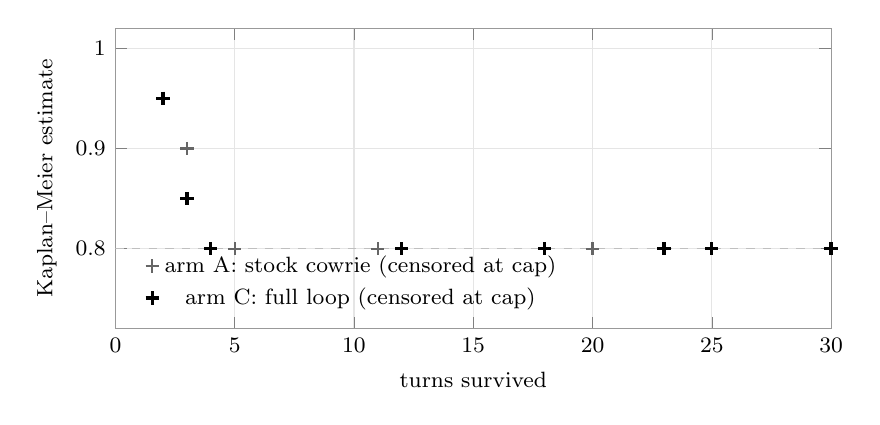
\begin{tikzpicture}
\begin{axis}[
  width=0.88\linewidth,
  height=5.4cm,
  xmin=0, xmax=30,
  ymin=0.72, ymax=1.02,
  xlabel={turns survived},
  ylabel={Kaplan--Meier estimate},
  xlabel style={font=\footnotesize},
  ylabel style={font=\footnotesize},
  tick label style={font=\footnotesize},
  legend style={font=\footnotesize, at={(0.03,0.03)}, anchor=south west, draw=none, fill=none},
  grid=major,
  grid style={black!10},
  axis line style={black!40},
]
% Arm A: stock cowrie
\addplot[
  color=black!60, thick, dash pattern=on 4pt off 2pt,
  mark=+, only marks, mark size=2.4,
  mark options={solid, black!60},
] coordinates {
  (2,0.95) (3,0.90) (4,0.80) (5,0.80) (11,0.80)
  (12,0.80) (18,0.80) (20,0.80) (25,0.80) (30,0.80)
};
\addlegendentry{arm A: stock cowrie (censored at cap)}
% Arm C: full loop
\addplot[
  color=black, very thick,
  mark=+, only marks, mark size=2.4,
  mark options={solid, black},
] coordinates {
  (2,0.95) (3,0.85) (4,0.80) (12,0.80) (18,0.80)
  (23,0.80) (25,0.80) (30,0.80)
};
\addlegendentry{arm C: full loop (censored at cap)}
\addplot[black!25, dashed, thin, domain=0:30] {0.80};
\end{axis}
\end{tikzpicture}
\caption{Kaplan--Meier estimates of turns survived under the v2
pre-registration ($n{=}20$ per arm, horizon 30, persona-scaled caps).
The curves coincide from turn 4 onward: every attacker still engaged at
turn 4 remains to the horizon, and 16 of 20 sessions per arm are censored
at their cap. Saturation, not separation, is the measured outcome
(\texttt{results/field\_attack/arm\_v2\_stats.json}).}
\label{fig:km}
\end{figure}

The primary endpoint (turns survived, 30-turn horizon) saturates
(Figure~\ref{fig:km}): 16 of 20 per arm at cap (RMST 24.65 vs 24.60;
log-rank $p=0.975$, Holm $p=1.0$). Saturation is the deception-floor
result---neither surface lost an attacker---but the design cannot
discriminate engagement beyond the cap. Bait capture is 0 of 20 per arm
(3 of 40 artifact reads---untested safety floor), again 0 of 10 per arm
with 10 reads under the disjoint-brain replication.

The one separating interval is the clearest signature a generative
surface produces: planted artifacts appeared in 11 of 20 RAGIN-arm
transcripts vs 0 of 20 on stock ($p=0.00015$)---exploratory there, then
promoted to primary in a third pre-registered contrast under a
family-disjoint brain (claude-sonnet-5-5, Anthropic family, vs the
OpenAI serving generator; $n{=}10$ per arm). The signature replicates
confirmatorily: 6 of 10 RAGIN sessions returned planted artifacts vs 0
of 10 stock (Fisher $p=0.011$; specific shapes 5 of 10, $p=0.033$; RD
$0.60$, case-level CI $[0.30, 0.90]$). Two failures reported
symmetrically: bait capture again 0 of 10 per arm (10 of 20 reads,
never reused), and the detection persona fingerprints both surfaces
equally (two \texttt{VERDICT: honeypot} verdicts per arm). A direct
control locates the mechanism: bait files planted into stock cowrie
remain unserved (static honeyfs binds the file map at startup), while
the fiction ledger serves content without restart---the contrast
measures dynamic serving capability stock surfaces structurally lack
(\path{results/field_attack_v3/arm_v3_stats.json}).

Three caveats: local self-play, shared endpoint, surfaces differ by
design. No per-arm endpoint survives the pre-registered correction
(\S\ref{sec:labels}).

\subsection{Label Provenance and Rating Disclosure}
\label{sec:labels}
The 120-case confirmatory packet behind the composite of
\S\ref{sec:rq3} is labeled here by a disclosed AI panel, not by people.
Three checkpoints from one model family (\texttt{gpt-5.6-sol},
\texttt{gpt-6-astra}, \texttt{gpt-6.1-sol}) each label every case
independently, blind to arm and to one another, under the verbatim
operational definitions of the frozen taxonomy, in a per-model
deterministic case order
(\path{results/laya_research/ai_jury_v1/ai_jury_manifest.json}); a separate 218-row audit with three independently served raters
reaches $\kappa=0.866$ on identification, $1.0$ at family level (F1
$0.732$ strict; all technique conflicts trace to echo text)
(\path{results/cti_manual_audit.json}). The panel
reaches Fleiss $\kappa=0.811$ over nine classes, pairwise exact agreement
$0.900$--$0.958$, and $0.967$--$0.975$ on the malicious/benign collapse; the full label
distribution is disclosed (273/360 benign) so chance correction can be
audited. A case-level bootstrap bounds panel $\kappa$ at $[0.714, 0.896]$ (binary $[0.848, 0.984]$; leave-one-out $0.764$--$0.897$, \path{results/laya_research/ai_jury_bootstrap_ci/}). We report this as an AI-workload reliability
check under a declared protocol. It is not a human study, and no human-labelled packet exists in this
release. All three checkpoints share one provider family; a disjoint-family juror (claude-sonnet-5-5) labeling 118 of the 120
packet cases (two unresolved by provider quota) agrees with each GPT
checkpoint at $0.76$--$0.81$ exact ($0.86$--$0.88$
binary), and adding it drops panel $\kappa$ from $0.805$ to $0.675$
(binary $0.922$ to $0.795$)---the correlated-error mass, previously
invisible, is measured, not assumed. The previously archived
r1--r3 packets are model-produced and are not used as ground truth.

Why an AI-judged lane is correct here: the estimand is
machine-vs-machine fidelity---whether the deception withstands the
AI-attacker population generating the workload. Subjects and judged
objects are both machine artifacts, so independent AI raters, blind to
arm and order and served off the pipeline, are the matching instrument.
Three additional arguments bound the case for human raters as gold
standard. First, the deployment population for this class of deception
is itself automated (scanner bots, AI-attacker tooling): a human panel
would measure human susceptibility, not the quantity the deployment
confronts. Second, by 2026 the human-versus-AI labeling distinction is
operationally blurred---practicing CTI analysts use AI-assisted tooling
for triage and enrichment, so a "human-labeled" ground truth already
embeds the same model families this paper discloses. Third, the
matching-instrument argument does not claim AI raters are better than
humans; it claims they measure the quantity the deployment actually
faces. We claim reliability under a declared protocol, not validity;
the probes below bound where it holds.

A deterministic reference makes the ceiling visible: a structural
labeler (command heads, credential paths, persistence verbs) labels the
same cases without a model, agreeing with the panel majority on $50.8\%$
exactly (binary $\kappa=0.317$; 30 cases outside its rules). The
disagreement concentrates on the benign/recon boundary---intent, which
neither a rule set nor a single shell command carries
(\path{results/laya_research/ai_jury_oracle_v1/oracle_agreement.json}). The composite
is therefore reported as contract compliance under declared operational
definitions, and the rater line of \S\ref{sec:advworkload} is a protocol
for future validation rather than a claim of this paper.

A second probe measures the protocol: two paraphrases of the same
definitions relabel the same 120 cases---each checkpoint reproduces
$0.81$--$0.97$ of its own baseline labels, but panel $\kappa$ moves to
$0.790$ and $0.663$, so the $\kappa=0.811$ headline is a property of the
wording as well as the evidence; cross-family juror labels for the same
packet are packaged alongside (\path{results/panel_v3/}).

\subsection{Adversarial Hardening of the Serving Path}
\label{sec:hardening}
Two red-team waves targeted the serving system itself, complementing
the verifier battery (\S\ref{sec:rq2} and Supplement
\S\ref{app:probes}). Wave~1 probed the serving layer with live HTTP replays plus a
verification-gate payload battery and found eleven vulnerabilities, each
closed behind a regression test (96 new unit tests; the suite grew 1992
to 2088): a cross-attacker session takeover, a whole-honeypot freeze (one
20-KB command held a global lock for 110~s; now sharded with compiled
alternations), an unauthenticated \texttt{/health} fingerprint dump, an
unbounded transcript map pinning 16.8~GB (now byte-budgeted), session-id
traversal, an mTLS boot-order gap, non-constant-time key comparison,
missing 413, and 500s on closed sessions (now fail-closed 503). On the gate, 12 of 15 real secret
shapes used to bypass the danger check; after the repair, 0 of 11
attack payloads bypass it, including a hardened NFKC plus zero-width
view over the whole battery and command-shaped transports. API-key
auth, mTLS layering, path normalization, and the fail-closed serving
discipline held under every probe---no unverified text was served in
any of them---and the deception fiction behaved identically before
and after: the verifier red-team artifacts still pass all 47
consistency checks, and the 89-case live authored battery stands at
precision 0.994 and recall 0.943.

Wave~2 attacked the pipeline and control chain (data-pipeline
injection, LLM/JEV-chain abuse, crypto and configuration): 14 of 16
findings fixed behind 42 regression tests, plus the crypto HIGH
(audit-integrity rows were signed with a git-tracked default HMAC key,
making tamper evidence forgeable) now failing closed with no default
key (8 dedicated tests). A secrets-in-tree scan comes back clean, and
three MEDIUM findings are deferred with written rationale rather than
silently dropped.
